% ===================================================================
%  Adaptive Cyber-Physical Intrusion Detection System:
%  A Multi-Tier Hybrid Architecture Combining Supervised Learning,
%  Deep Anomaly Detection, and Latent-Space Ensemble Fusion
%  IEEE Two-Column Journal/Conference Paper
%
%  Compile (from the report/ directory):
%    pdflatex --shell-escape combined_main.tex
%    bibtex combined_main
%    pdflatex --shell-escape combined_main.tex
%    pdflatex --shell-escape combined_main.tex
% ===================================================================
\documentclass[10pt,journal,compsoc]{IEEEtran}

% ---- Core packages ----
\usepackage[T1]{fontenc}
\usepackage[utf8]{inputenc}
\usepackage{graphicx}
\usepackage{svg}
\usepackage{booktabs}
\usepackage{amsmath}
\usepackage{amssymb}
\usepackage{float}
\usepackage{caption}
\captionsetup{font=small, skip=3pt}
\usepackage{xcolor}
\usepackage{enumitem}
\usepackage{cite}
\usepackage{url}
\usepackage{microtype}
\usepackage{balance}
\usepackage{multirow}
\usepackage{array}
\usepackage{algorithm}
\usepackage{algpseudocode}
\usepackage{tabularx}

\usepackage[colorlinks=true,
            linkcolor=blue,
            citecolor=blue,
            urlcolor=blue,
            pdftitle={Adaptive CPS IDS: Multi-Tier Hybrid Architecture},
            pdfauthor={Pugazhendhi J and Dally R}]{hyperref}

% ---- Graphics path (compile from report/) ----
\graphicspath{{../}}

% ---- Float/caption spacing ----
\setlength{\floatsep}{4pt plus 1pt minus 1pt}
\setlength{\textfloatsep}{6pt plus 2pt minus 2pt}
\setlength{\intextsep}{4pt plus 1pt minus 1pt}
\setlength{\dblfloatsep}{4pt plus 1pt minus 1pt}
\setlength{\dbltextfloatsep}{6pt plus 2pt minus 2pt}
\setlength{\abovecaptionskip}{3pt}
\setlength{\belowcaptionskip}{1pt}

% ---- Title ----
\title{Adaptive Cyber-Physical Intrusion Detection:\\A Multi-Tier Hybrid Architecture Combining\\Supervised Learning, Deep Anomaly Detection,\\and Latent-Space Ensemble Fusion}

\author{
  \IEEEauthorblockN{Pugazhendhi J}
  \IEEEauthorblockA{
    \textit{Department of CS and AI}\\
    Rishihood University, Sonipat, India\\
    \href{mailto:pugazhendhi.j23csai@nst.rishihood.edu.in}
         {pugazhendhi.j23csai@nst.rishihood.edu.in}}
  \and
  \IEEEauthorblockN{Dally R}
  \IEEEauthorblockA{
    \textit{Department of CS and AI}\\
    Rishihood University, Sonipat, India\\
    \href{mailto:dally.r23csai@nst.rishihood.edu.in}
         {dally.r23csai@nst.rishihood.edu.in}}
}

\IEEEspecialpapernotice{(Extended Research Article)}

% ===================================================================
\begin{document}
\maketitle

% ---- Abstract ----
\begin{abstract}
Modern cyber-physical systems (CPS) operate in open-world environments
where both known and previously unseen (zero-day) network threats must
be detected with high confidence and minimal false alarms.  Purely
supervised classifiers achieve near-perfect precision on known attack
families but deliver zero recall against novel threats, while
unsupervised anomaly detectors generalize at the cost of precision.
This paper presents \textbf{AdaptiveIDS}, a comprehensive, multi-tier
intrusion detection architecture evaluated on the full CIC-IDS-2018
benchmark (8{,}284{,}195 network flows, 13 attack families) that
systematically bridges this precision-recall divide.  The architecture
progresses from a supervised Random Forest (RF) baseline with perfect
precision on known attacks, through a One-Class SVM (OC-SVM) providing
initial zero-day coverage, to a deep Autoencoder (AE) family offering
continuous anomaly scoring via reconstruction-error thresholding, and
finally to six hybrid models that couple learned AE latent
representations with explicit boundary classifiers in a 32-dimensional
bottleneck space.  Three AE variants are evaluated: a standard AE
(ROC-AUC 0.8965), a Sparse AE with L1 activity regularization
(ROC-AUC 0.8929), and a Denoising AE with Gaussian input corruption
(ROC-AUC 0.8867, F1 0.1433, Precision 0.8179).  An ablation study
reveals that Denoising AE training is the single most impactful
design decision (+327\% F1 over the standard baseline), while coupling
boundary classifiers (OC-SVM, Isolation Forest) directly in the
bottleneck space degrades AUC by 0.42--0.47 points due to overlapping
latent distributions.  The AE + RF pseudo-label hybrid uniquely
maintains competitive AUC (0.7920) by operating in the original
feature space, demonstrating a neuro-symbolic synergy where the
neural component bootstraps the symbolic learner (+131\% AUC over an
unaided RF).  The central finding is that \emph{representation quality}
is the limiting bottleneck: deep noise-robust autoencoders, not
ensemble fusion, are the recommended path to open-world CPS security.
\end{abstract}

\begin{IEEEkeywords}
Intrusion Detection System, CIC-IDS-2018, Random Forest, One-Class SVM,
Autoencoder, Sparse Autoencoder, Denoising Autoencoder, Isolation Forest,
Hybrid IDS, Meta-Ensemble, Zero-Day Detection, Anomaly Detection,
Cyber-Physical Security, Deep Learning, Latent Space, Neuro-Symbolic
\end{IEEEkeywords}

% ===================================================================
\section{Introduction}
\label{sec:intro}

Cyber-physical systems underpin critical infrastructure---smart grids,
industrial control systems, autonomous vehicles, and medical
devices---that must operate continuously under adversarial conditions
\cite{raza2013svelte}.  Traditional intrusion detection systems (IDS)
follow a signature-based paradigm: predefined rules or supervised
classifiers identify known attack patterns with high precision but are
fundamentally blind to novel, zero-day threats
\cite{liao2013intrusion, sommer2010outside}.  As attack surfaces
expand and adversaries continuously evolve their techniques, this
closed-world assumption is increasingly untenable for production CPS
deployments.

Anomaly-based IDS approaches address the zero-day gap by learning a
model of normal behavior and flagging statistical deviations
\cite{garcia2009anomaly}.  However, the precision-recall trade-off
inherent to anomaly detection---high recall at the cost of elevated
false positive rates---limits operational deployability in environments
where alert fatigue is a real constraint.  The central research
question motivating this work is: \emph{how can we maximally reduce
the precision-recall gap for both known and unknown attacks in a
unified, deployable architecture?}

This paper makes the following contributions:

\begin{enumerate}[leftmargin=*,noitemsep,topsep=2pt]
  \item \textbf{Comprehensive Baseline Evaluation.}  We establish
    rigorous supervised (RF) and semi-supervised (OC-SVM) baselines
    on the full CIC-IDS-2018 dataset \cite{sharafaldin2018}, the
    largest publicly available network intrusion benchmark, with a
    systematic zero-day evaluation protocol.
  \item \textbf{Deep AE Anomaly Scoring.}  We design and evaluate
    three Autoencoder variants---Standard, Sparse, and
    Denoising---trained exclusively on benign traffic, providing
    continuous, threshold-tunable anomaly scores with per-attack
    diagnostic profiling.
  \item \textbf{Hybrid Latent-Space Models.}  We couple AE bottleneck
    representations with OC-SVM, Isolation Forest, and pseudo-label RF
    boundary classifiers, producing six hybrid configurations.  We
    demonstrate both the conditions under which hybridization succeeds
    (RF in the original feature space) and when it fails (boundary
    models in the compressed latent space).
  \item \textbf{Meta-Ensemble Analysis.}  We evaluate equal-weight
    score-level fusion of all eight component anomaly scores, identify
    the score-dilution failure mode, and quantify the contribution of
    each component via a systematic ablation study.
  \item \textbf{Operational Recommendations.}  We derive concrete
    deployment guidance for CPS operators, including threshold
    selection criteria and a tiered alerting strategy.
\end{enumerate}

The remainder of this paper is organized as follows.
Section~\ref{sec:related} surveys related work.
Section~\ref{sec:dataset} describes the dataset and preprocessing
pipeline.  Section~\ref{sec:arch} presents the system architecture.
Section~\ref{sec:method} details each model family and fusion
strategy.  Section~\ref{sec:exp} defines the evaluation protocol.
Section~\ref{sec:results} presents comprehensive experimental results.
Section~\ref{sec:ablation} provides the ablation study.
Section~\ref{sec:innovation} analyzes hybrid innovation.
Section~\ref{sec:discussion} discusses operational implications.
Section~\ref{sec:repro} addresses reproducibility.
Section~\ref{sec:limits} covers limitations and future work, and
Section~\ref{sec:conclusion} concludes.

% ===================================================================
\section{Related Work}
\label{sec:related}

\subsection{Signature-Based and Supervised IDS}

Early IDS research relied on hand-crafted rule sets, which were later
supplanted by machine learning approaches.  Breiman's Random Forest
\cite{breiman2001} emerged as a dominant supervised baseline due to
its resistance to overfitting and native feature importance estimation.
Evaluations on the KDD Cup 1999 \cite{tavallaee2009nsl} and
CICIDS-2017/2018 \cite{sharafaldin2018} datasets confirmed RF's
near-perfect performance on known attack families.  However, as
Sommer and Paxson \cite{sommer2010outside} argued, supervised
classifiers trained on closed-world datasets cannot generalize to
the open-world conditions of real deployments.

\subsection{Anomaly-Based and Semi-Supervised Detection}

One-Class SVM (OC-SVM) \cite{scholkopf2001} models a minimum-volume
hypersphere around the support of the training (benign) distribution,
declaring points outside the sphere as anomalies.  This approach
provides non-zero zero-day recall by construction but suffers from
quadratic training complexity and sensitivity to the $\nu$
hyperparameter.  Chandola et al. \cite{chandola2009} survey the
broader anomaly detection landscape, concluding that no single method
dominates across all evaluation regimes.

\subsection{Deep Learning for IDS}

Convolutional neural networks \cite{kim2020cnn, sensors2023} and
autoencoders \cite{mirsky2018kitsune, vincent2010} have demonstrated
strong performance on network intrusion benchmarks.  Autoencoders
trained on benign-only data exploit the reconstruction-error gap
between normal and anomalous flows \cite{hinton2006}.  The Kitsune
system \cite{mirsky2018kitsune} demonstrated online, ensemble-of-AE
anomaly detection in production network environments.  Our work
extends this direction by evaluating sparse and denoising AE variants
and coupling them with explicit boundary classifiers in the learned
latent space.

\subsection{Hybrid and Ensemble IDS}

Buczak and Guven \cite{buczak2016} survey ML methods for
cybersecurity, identifying ensemble approaches as consistently superior
to single-model baselines.  Dietterich \cite{dietterich2000}
theoretically motivates ensemble diversity as the source of
performance gains, a principle we test empirically for the score-level
fusion case.  Recent work \cite{plosone2024, ijsse2025} confirms that
hybrid architectures must address both known and unknown attacks to be
deployment-ready, but few papers systematically study when coupling
deep representations with classical boundary models helps versus hurts.
This gap motivates our hybrid evaluation framework.

% ===================================================================
\section{Dataset and Preprocessing}
\label{sec:dataset}

\subsection{CIC-IDS-2018}

All experiments use the Canadian Institute for Cybersecurity
CIC-IDS-2018 dataset \cite{sharafaldin2018}, captured over five days
(February 14--23, 2018) across a 50-machine victim network.  The raw
dataset contains 8{,}284{,}195 labeled network flows spanning one
benign class and 13 distinct attack families:

\begin{itemize}[leftmargin=*,noitemsep]
  \item \textbf{Denial of Service:} DoS-Hulk, DoS-Slowloris,
        DoS-SlowHTTPTest, DoS-GoldenEye
  \item \textbf{Distributed DoS:} DDoS attacks
  \item \textbf{Brute Force:} SSH-Patator, FTP-Patator
  \item \textbf{Web Attacks:} SQL Injection, XSS, Brute Force
  \item \textbf{Infiltration:} ARES RAT-based infiltration
  \item \textbf{Botnet:} ARES botnet
\end{itemize}

CIC-IDS-2018 is preferred over the older KDD Cup 1999 and NSL-KDD
datasets \cite{tavallaee2009nsl} because it reflects contemporary
attack tools, uses modern network protocols, and provides raw PCAP
files enabling reproducible feature extraction.

\subsection{Feature Extraction and Engineering}

Raw PCAPs are processed using CICFlowMeter to yield 80 bidirectional
flow features per record.  We apply the following preprocessing
pipeline:

\begin{enumerate}[leftmargin=*,noitemsep,topsep=2pt]
  \item \textbf{ID removal:} Drop timestamp, source/destination IP,
        and port columns (non-generalizable identifiers).
  \item \textbf{Type coercion:} Force all columns to \texttt{float32};
        non-numeric values are coerced to \texttt{NaN}.
  \item \textbf{Imputation:} Replace \texttt{NaN} and \texttt{Inf}
        values with zero.
  \item \textbf{Constant-column removal:} Drop features with zero
        variance across the training split.
  \item \textbf{Correlation pruning:} Remove one member of each pair
        of features with Pearson $|\rho| > 0.98$, eliminating
        redundant feature dimensions.
  \item \textbf{Robust scaling:} Apply \texttt{RobustScaler}
        (median/IQR normalization) to reduce sensitivity to outliers.
\end{enumerate}

After preprocessing, 68 numeric features remain.  The final modeling
dataset contains 3{,}215{,}110 flows: 2{,}050{,}783 benign
(63.8\%) and 1{,}164{,}327 attack (36.2\%).  All cached arrays are
reproducible with \texttt{SEED=42}.

\subsection{Zero-Day Evaluation Protocol}

To evaluate generalization to unseen attack families, we establish a
\emph{seen/unseen split}: the supervised RF is trained on benign
traffic plus a single attack family (\texttt{dos attacks-hulk}) as
the positive class, while all other attack families are withheld as
zero-day threats during threshold evaluation.  Anomaly detectors are
trained on benign-only subsets; all attack flows are treated as
zero-day by design.  The 99th percentile of benign validation errors
($P_{99}$) serves as the default anomaly threshold for all threshold-
dependent metrics.

% ===================================================================
\section{System Architecture}
\label{sec:arch}

Figure~\ref{fig:arch_overview} illustrates the complete end-to-end
architecture of AdaptiveIDS.  The system processes raw network traffic
through a shared preprocessing pipeline and then routes flows through
three functional tiers operating in parallel.

\begin{figure*}[t!]
\centering
\includesvg[width=\linewidth,inkscapelatex=false]{../adaptive_ids_full_architecture}
\caption{End-to-end AdaptiveIDS architecture.  \textbf{Tier~1} (left)
  is a supervised Random Forest that identifies known attack families
  with 100\% precision.  \textbf{Tier~2/3} (right) encompasses three
  Autoencoder variants (Standard, Sparse, Denoising) that compress
  traffic into a 32-dimensional latent bottleneck.  Boundary
  classifiers (OC-SVM, Isolation Forest, RF pseudo-label) draw
  explicit decision surfaces in this latent space.  All eight normalized
  anomaly scores are aggregated by the \textbf{Meta-Ensemble} to
  yield the final IDS decision.  Score widths (thickness) conceptually
  represent discriminative quality; AE channels are stronger than
  bottleneck boundary channels.}
\label{fig:arch_overview}
\end{figure*}

\textbf{Tier~1 — Supervised Detection.}  A Random Forest classifier
trained on benign and known-attack traffic provides high-confidence,
interpretable detection for previously observed threat signatures.
Its output is a binary label (known attack / benign).

\textbf{Tier~2 — Deep Representation Learning.}  Three AE variants
encode all traffic (labeled and unlabeled) into a 32-dimensional
latent bottleneck.  The bottleneck is the shared representation space
used both for reconstruction-error anomaly scoring and as input to
Tier~3 boundary classifiers.

\textbf{Tier~3 — Latent-Space Boundary Modeling.}  OC-SVM and
Isolation Forest are trained on benign bottleneck vectors to draw
explicit decision surfaces in the compressed space.  A pseudo-label
RF uses AE-generated anomaly labels to train a discriminative
classifier in the original feature space.

\textbf{Meta-Ensemble.}  All eight component anomaly scores are
min-max normalized to $[0,1]$ and averaged with equal weight to
produce a single ensemble anomaly score.

% ===================================================================
\section{Methodology}
\label{sec:method}

\subsection{Tier 1 — Random Forest Classifier}

A Random Forest \cite{breiman2001} with 100 decision trees is trained
on 70\% of the binary-labeled subset (benign vs.\ \texttt{dos
attacks-hulk}).  Hyperparameters: \texttt{max\_features=sqrt},
\texttt{min\_samples\_leaf=1}, \texttt{class\_weight=balanced}.
Feature importance is computed via mean decrease in impurity, providing
an interpretable ranking of the 68 input features.

\subsection{Tier 2 — Autoencoder Family}

All three AE variants share a common encoder-decoder skeleton:
\begin{equation}
  \mathbf{68} \!\to\! \mathbf{128} \!\to\! \mathbf{64}
  \!\to\! \boldsymbol{32} \!\to\! \mathbf{64}
  \!\to\! \mathbf{128} \!\to\! \mathbf{68}
\end{equation}
with batch normalization after each dense layer, ReLU activations, and
20\% dropout.  All AEs are trained exclusively on benign flows using
the Adam optimizer ($\eta = 10^{-3}$, $\beta_1=0.9$, $\beta_2=0.999$)
for up to 50 epochs with early stopping (patience~7) and learning-rate
reduction on plateau (factor~0.5, patience~3).

\subsubsection{Standard Autoencoder}
Minimizes mean squared reconstruction error:
\begin{equation}
  \mathcal{L}_{\text{AE}} = \frac{1}{n}\sum_{i=1}^{n}
    \|\mathbf{x}_i - \hat{\mathbf{x}}_i\|^2.
\end{equation}
The reconstruction error $e_i = \|\mathbf{x}_i - \hat{\mathbf{x}}_i\|^2$
serves as the anomaly score: flows that deviate from the learned
benign manifold exhibit elevated errors.

\subsubsection{Sparse Autoencoder}
Adds L1 activity regularization on the bottleneck layer:
\begin{equation}
  \mathcal{L}_{\text{SAE}} = \mathcal{L}_{\text{AE}}
    + \lambda\|\mathbf{z}\|_1, \quad \lambda = 10^{-4},
\end{equation}
where $\mathbf{z} \in \mathbb{R}^{32}$ is the bottleneck activation.
Sparsity encourages disentangled, more linearly separable latent
representations, potentially improving downstream boundary classifiers.

\subsubsection{Denoising Autoencoder}
A Gaussian noise layer ($\sigma = 0.1$) corrupts the input during
training while targets remain clean \cite{vincent2010}:
\begin{equation}
  \tilde{\mathbf{x}} = \mathbf{x} + \boldsymbol{\epsilon},
  \quad \boldsymbol{\epsilon} \sim \mathcal{N}(\mathbf{0},
  \sigma^2 \mathbf{I}).
\end{equation}
The model must recover $\mathbf{x}$ from $\tilde{\mathbf{x}}$,
forcing the encoder to learn features robust to small perturbations.
Attack flows, which deviate substantially from the benign manifold,
exhibit disproportionately elevated reconstruction errors.

\subsection{Tier 3 — Boundary Classifiers}

\subsubsection{One-Class SVM}
An OC-SVM \cite{scholkopf2001} with RBF kernel
($\nu=0.05$, $\gamma$=\texttt{scale}) is trained on 80{,}000
subsampled benign bottleneck vectors.  The training-set cap is
imposed by the quadratic complexity $\mathcal{O}(n^2)$ of the
SVM kernel matrix.  The decision function value serves as a
continuous anomaly score.

\subsubsection{Isolation Forest}
An Isolation Forest \cite{liu2008} with 200 trees and
\texttt{contamination=0.05} is trained on the full benign bottleneck
set.  Anomaly score is derived from the average path length required
to isolate each point: shorter paths indicate anomalies.

\subsubsection{RF Pseudo-Label Classifier}
The standard AE's $P_{99}$ threshold is applied to all training
flows to generate binary pseudo-labels.  A pseudo-label RF (200 trees,
\texttt{max\_depth=12}, balanced class weights) is then trained on
the original 68-dim features using a 500{,}000-flow subsample.
This configuration uniquely operates outside the compressed bottleneck.

\subsection{Score Fusion}

For each hybrid, the AE reconstruction error and the boundary model's
anomaly score are independently min-max normalized to $[0,1]$:
\begin{equation}
  s^{\text{norm}} = \frac{s - s_{\min}}{s_{\max} - s_{\min}}.
\end{equation}
Hybrid scores are combined with equal weighting ($\alpha = 0.5$):
\begin{equation}
  s_{\text{hybrid}} = \alpha \cdot s_{\text{AE}}^{\text{norm}}
    + (1-\alpha) \cdot s_{\text{boundary}}^{\text{norm}}.
\end{equation}
The Meta-Ensemble averages all $N=8$ normalized component scores:
\begin{equation}
  s_{\text{ensemble}} = \frac{1}{N}\sum_{k=1}^{N}
    s_k^{\text{norm}}.
\end{equation}

\subsection{Summary of Evaluated Configurations}

\begin{enumerate}[leftmargin=*,noitemsep,topsep=2pt]
  \item \textbf{RF Baseline:} Supervised classifier (known-attack only).
  \item \textbf{OC-SVM Baseline:} Kernel anomaly detector (raw 68-dim).
  \item \textbf{Standard AE:} Reconstruction-error anomaly detector.
  \item \textbf{Sparse AE:} L1-regularized bottleneck AE.
  \item \textbf{Denoising AE (DAE):} Noise-robust AE.
  \item \textbf{H1 — AE + OC-SVM:} OC-SVM in Standard AE bottleneck.
  \item \textbf{H2 — AE + IF:} Isolation Forest in Standard AE bottleneck.
  \item \textbf{H3 — AE + RF:} RF on AE pseudo-labels (68-dim space).
  \item \textbf{H4 — Sparse AE + OC-SVM:} OC-SVM in Sparse AE bottleneck.
  \item \textbf{H5 — DAE + OC-SVM:} OC-SVM in Denoising AE bottleneck.
  \item \textbf{H6 — Meta-Ensemble:} Equal-weight avg of all 8 scores.
\end{enumerate}

% ===================================================================
\section{Experimental Setup}
\label{sec:exp}

\subsection{Hardware and Software Environment}

All experiments were conducted on an AWS EC2 \texttt{t3.large}
instance (Ubuntu~24.04, 8~GB RAM, 16~GB swap, 2~vCPUs) with
Python~3.12.3, TensorFlow~2.21.0, scikit-learn~1.8.0, NumPy~2.4.4,
and Pandas~3.0.2.  The \texttt{matplotlib} backend was set to
\texttt{Agg} for headless plot generation.

\subsection{Training/Validation/Test Splits}

\begin{itemize}[leftmargin=*,noitemsep]
  \item AEs are trained on 80\% of the 2{,}050{,}783 benign flows
        (1{,}640{,}626 training, 410{,}157 validation).
  \item Anomaly thresholds are calibrated at the 99th percentile
        ($P_{99}$) of validation reconstruction errors.
  \item All models are evaluated on the full mixed dataset
        (3{,}215{,}110 flows) to compute threshold-dependent metrics.
\end{itemize}

\subsection{Evaluation Metrics}

We report the following metrics, each addressing a distinct operational
concern:

\begin{itemize}[leftmargin=*,noitemsep]
  \item \textbf{ROC-AUC:} Threshold-free discriminative power.
  \item \textbf{Average Precision (AP):} Area under the
        precision-recall curve; robust to class imbalance.
  \item \textbf{F1-Score} at $P_{99}$: Harmonic mean of precision
        and recall at the default operating threshold.
  \item \textbf{Precision} at $P_{99}$: Fraction of flagged flows
        that are true attacks (alert fidelity).
  \item \textbf{Recall} at $P_{99}$: Fraction of true attack flows
        detected (coverage).
  \item \textbf{False Positive Rate (FPR):} Fraction of benign flows
        incorrectly flagged (operational overhead).
\end{itemize}


% ===================================================================
\section{Results}
\label{sec:results}

\subsection{Baseline Model Performance}

Table~\ref{tab:baseline} reports the supervised and semi-supervised
baselines.  The Random Forest achieves perfect precision (1.000) and
high F1 (0.850) on the \emph{known} attack family but delivers zero
recall on all other attack families---confirming the fundamental
closed-world limitation of purely supervised approaches.  The OC-SVM
partially addresses this gap: trained only on benign flows, it achieves
non-zero recall (0.040) across all attack families at the cost of lower
precision (0.660).

\begin{table}[htbp]
\centering
\caption{Supervised and semi-supervised baseline results}
\label{tab:baseline}
\begin{tabular}{lcccc}
\toprule
\textbf{Model} & \textbf{Precision} & \textbf{Recall} & \textbf{F1} & \textbf{Zero-Day R.} \\
\midrule
Random Forest   & 1.000 & 0.130 & 0.240 & $\approx$0.000 \\
One-Class SVM   & 0.660 & 0.040 & 0.070 & 0.040 \\
\bottomrule
\end{tabular}
\end{table}

\subsection{Comprehensive Model Comparison}

Table~\ref{tab:comparison} presents results for all eleven model
configurations.  The standalone AE variants dominate on ROC-AUC
($>$0.88), while all hybrid configurations that embed boundary
classifiers in the bottleneck space fall below AUC~0.50.

\begin{table*}[htbp]
\centering
\caption{Comprehensive model comparison at the $P_{99}$ threshold.
  H1--H6 denote the six hybrid configurations.
  $\dagger$ = operates in original 68-dim feature space.}
\label{tab:comparison}
\begin{tabular}{lcccccc}
\toprule
\textbf{Model} & \textbf{ROC-AUC} & \textbf{Avg Prec.} & \textbf{F1} & \textbf{Recall} & \textbf{Precision} & \textbf{Accuracy} \\
\midrule
Standard AE (baseline)      & 0.8965 & 0.7578 & 0.0336 & 0.0174 & 0.5012 & 0.6379 \\
Sparse AE                   & 0.8929 & 0.7597 & 0.0336 & 0.0174 & 0.4986 & 0.6378 \\
\textbf{Denoising AE (DAE)} & \textbf{0.8867} & \textbf{0.7675} & \textbf{0.1433} & \textbf{0.0785} & \textbf{0.8179} & \textbf{0.6600} \\
H1: AE + OC-SVM             & 0.4600 & 0.3137 & 0.0094 & 0.0048 & 0.2127 & 0.6332 \\
H2: AE + Isolation Forest   & 0.4231 & 0.3392 & 0.0116 & 0.0060 & 0.2508 & 0.6336 \\
H3: AE + RF$^\dagger$       & 0.7920 & 0.5593 & 0.0335 & 0.0174 & 0.4976 & 0.6378 \\
RF alone$^\dagger$           & 0.3433 & 0.3176 & 0.0335 & 0.0173 & 0.4978 & 0.6378 \\
H4: Sparse AE + OC-SVM      & 0.4206 & 0.3007 & 0.0190 & 0.0098 & 0.3561 & 0.6350 \\
H5: DAE + OC-SVM            & 0.4783 & 0.3186 & 0.0057 & 0.0029 & 0.1398 & 0.6325 \\
H6: Meta-Ensemble           & 0.4140 & 0.3024 & 0.0098 & 0.0050 & 0.2202 & 0.6332 \\
\bottomrule
\end{tabular}
\end{table*}

\subsection{ROC and Precision-Recall Curves}

Figures~\ref{fig:roc_all} and~\ref{fig:pr_all} visualize the
threshold-free discriminative performance.  The three AE variants
cluster near the upper-left corner (AUC $>0.88$), while all
OC-SVM/IF hybrid curves hug the random-baseline diagonal (AUC~$\approx
0.43$--$0.48$), consistent with the overlapping latent distributions
hypothesis discussed in Section~\ref{sec:analysis}.

\begin{figure}[htbp]
\centering
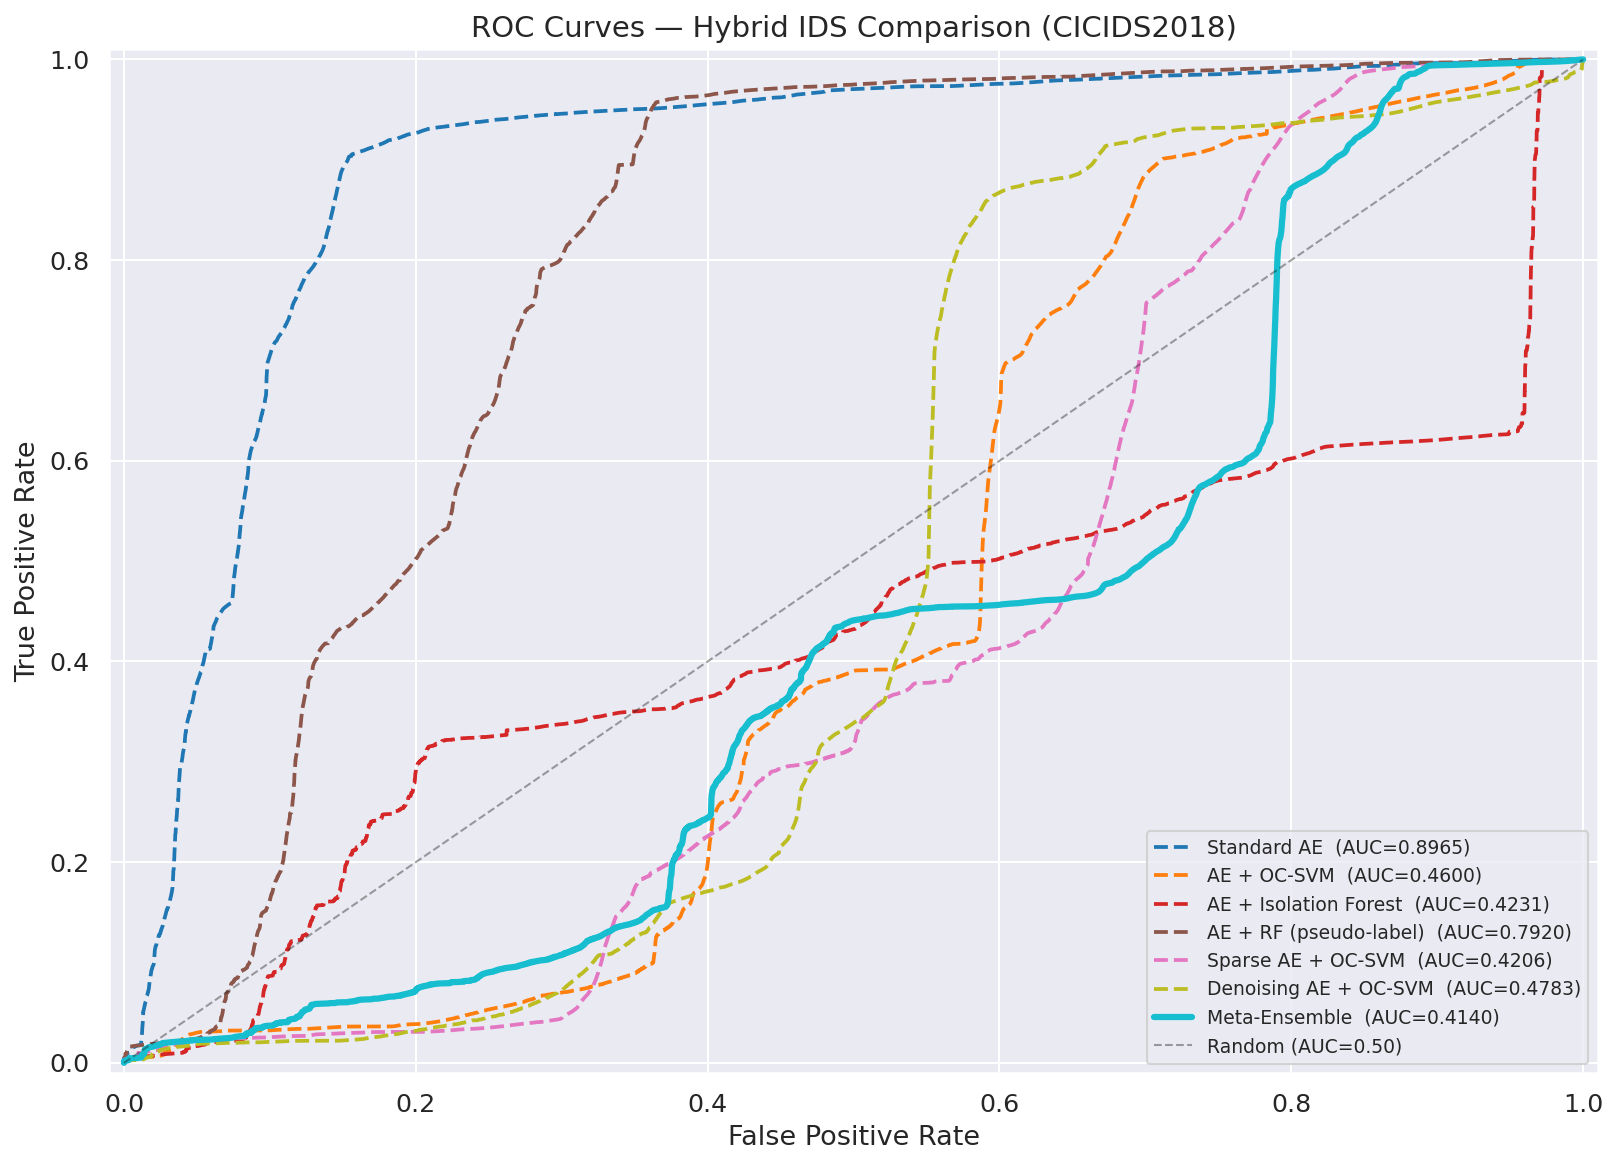
\includegraphics[width=\linewidth]{outputs/plots/models/hybird_output/plot_roc_all_models.png}
\caption{ROC curves for all hybrid IDS configurations.  Standalone AE
  variants cluster near the upper-left corner (AUC $>$0.88); hybrid
  models with OC-SVM/IF in the bottleneck space perform near or below
  the random baseline.}
\label{fig:roc_all}
\end{figure}

\begin{figure}[htbp]
\centering
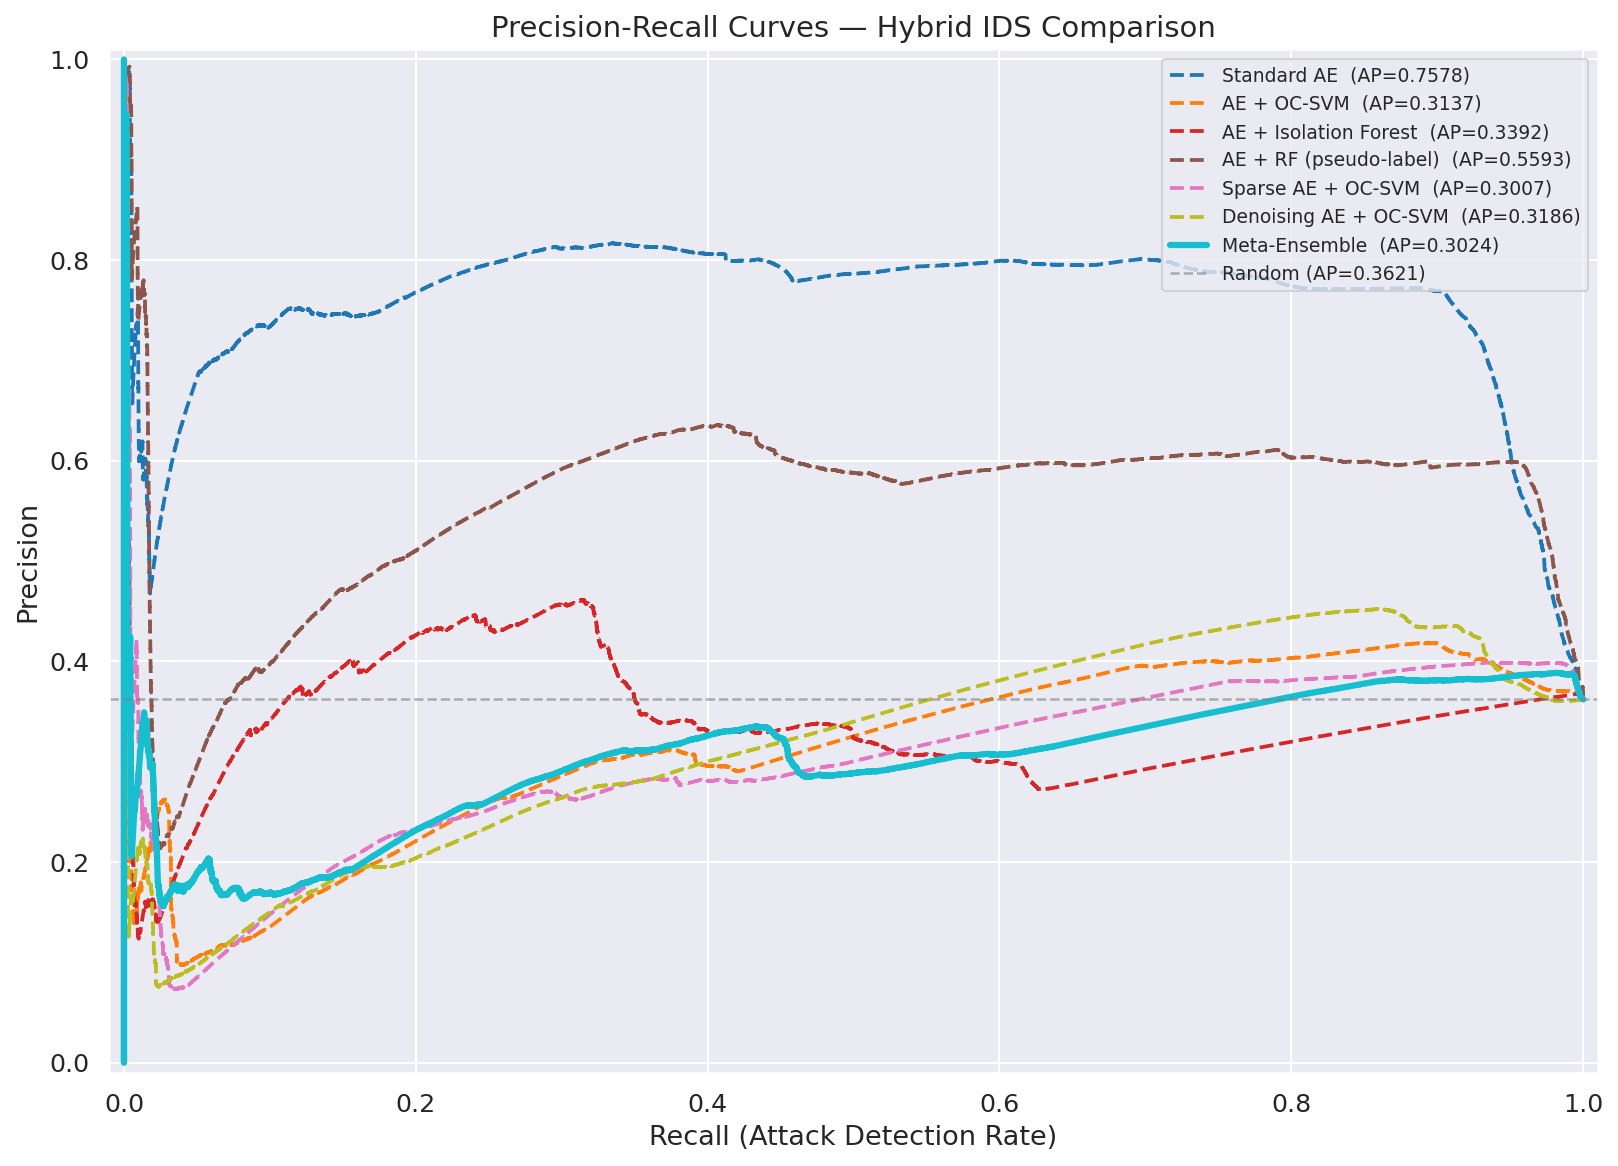
\includegraphics[width=\linewidth]{outputs/plots/models/hybird_output/plot_pr_all_models.png}
\caption{Precision-Recall curves for all models.  The Denoising AE
  achieves the highest average precision (0.7675), followed by the
  Sparse AE (0.7597) and Standard AE (0.7578).}
\label{fig:pr_all}
\end{figure}

\subsection{Metric Bar Comparison}

Figure~\ref{fig:metric_bar} provides a direct visual comparison of
F1, ROC-AUC, and Recall across all configurations, highlighting the
performance gap between the AE family and hybrid models.

\begin{figure}[htbp]
\centering
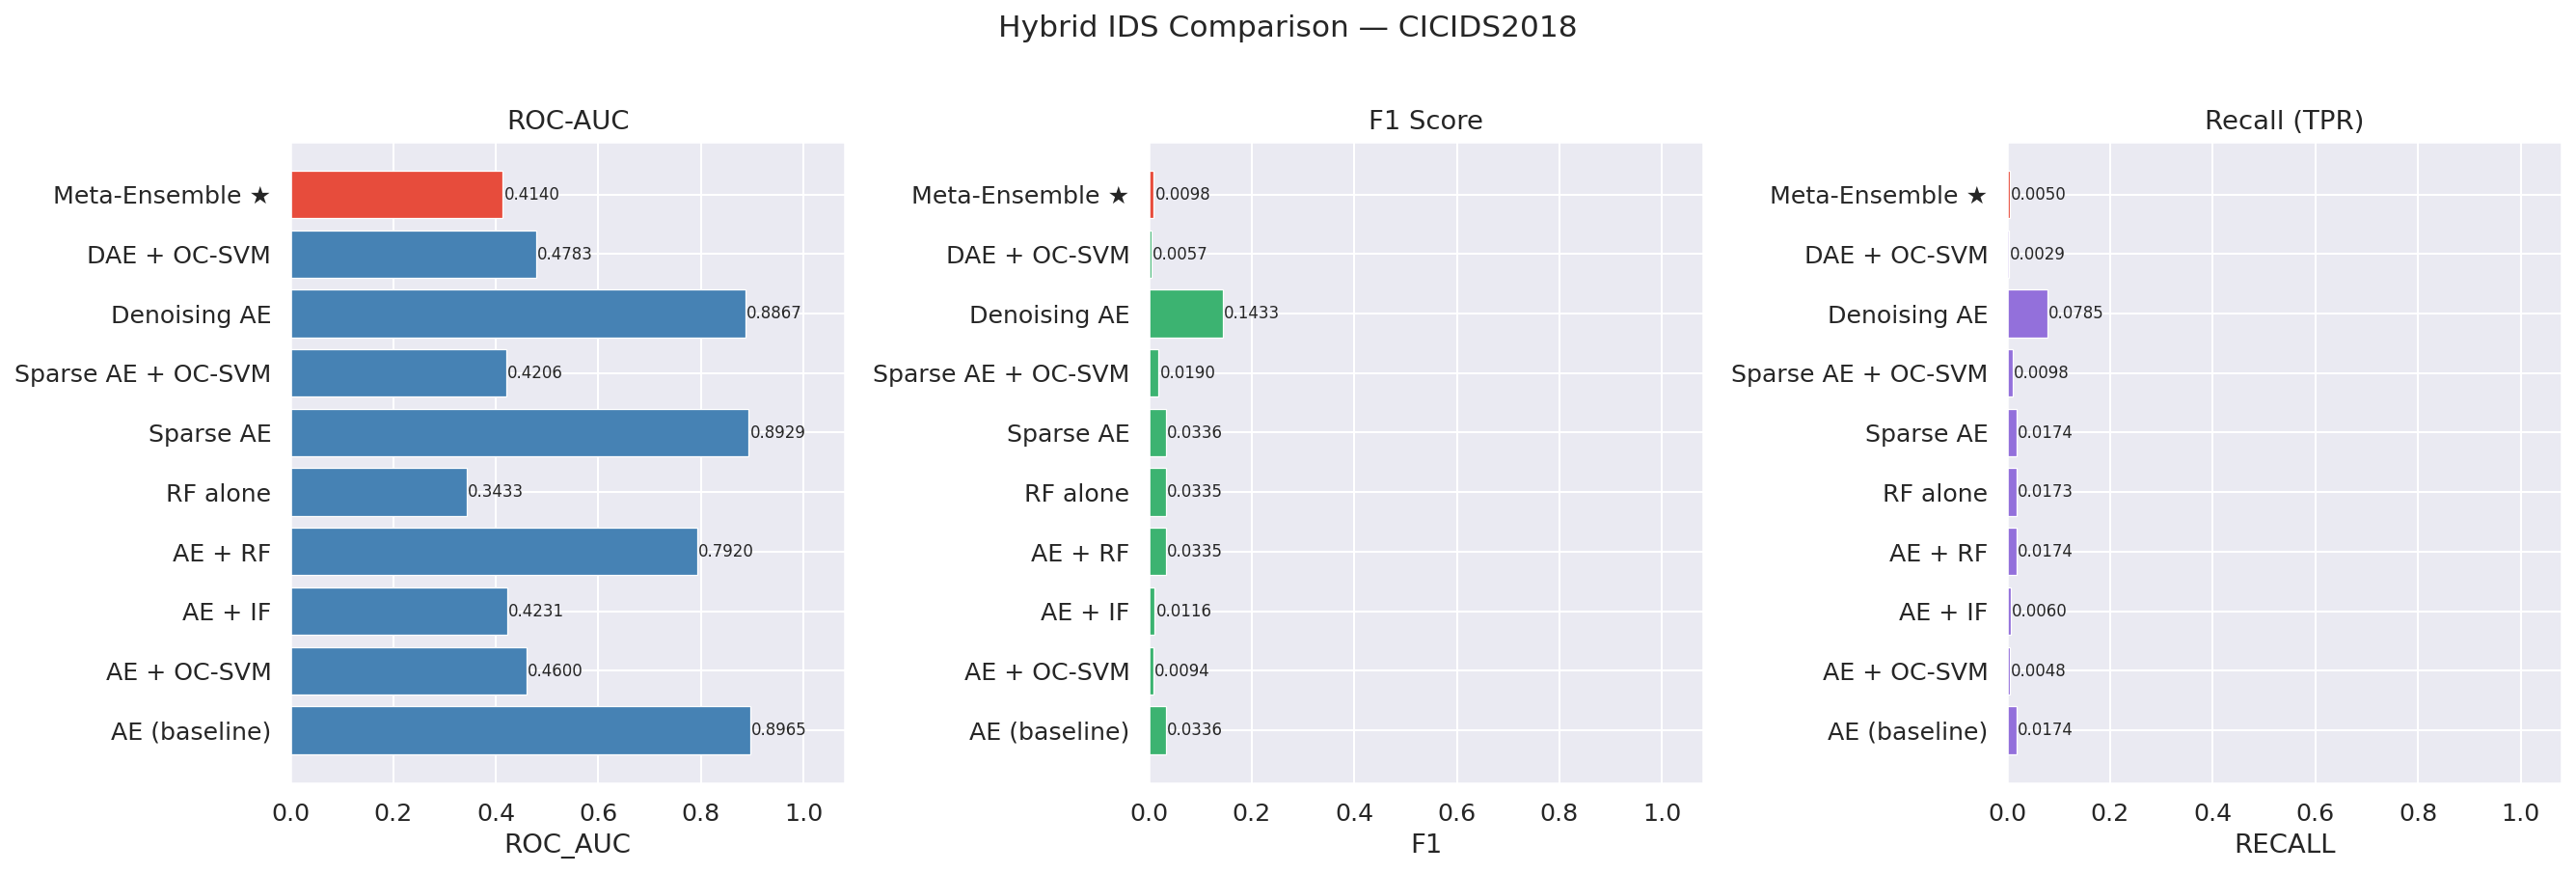
\includegraphics[width=\linewidth]{outputs/plots/models/hybird_output/plot_metric_comparison.png}
\caption{F1, ROC-AUC, and Recall comparison.  Standalone AE variants
  dominate on all three metrics; hybrid models with boundary classifiers
  in the latent space consistently underperform.}
\label{fig:metric_bar}
\end{figure}

\subsection{Meta-Ensemble Confusion Matrix}

Figure~\ref{fig:cm_ensemble} shows the Meta-Ensemble confusion matrix
at the $P_{99}$ threshold.  Of 1{,}164{,}327 true attack flows,
only 5{,}842 are detected (recall $\approx$0.005) while 20{,}690
benign flows are falsely flagged (precision 0.2202).

\begin{figure}[htbp]
\centering
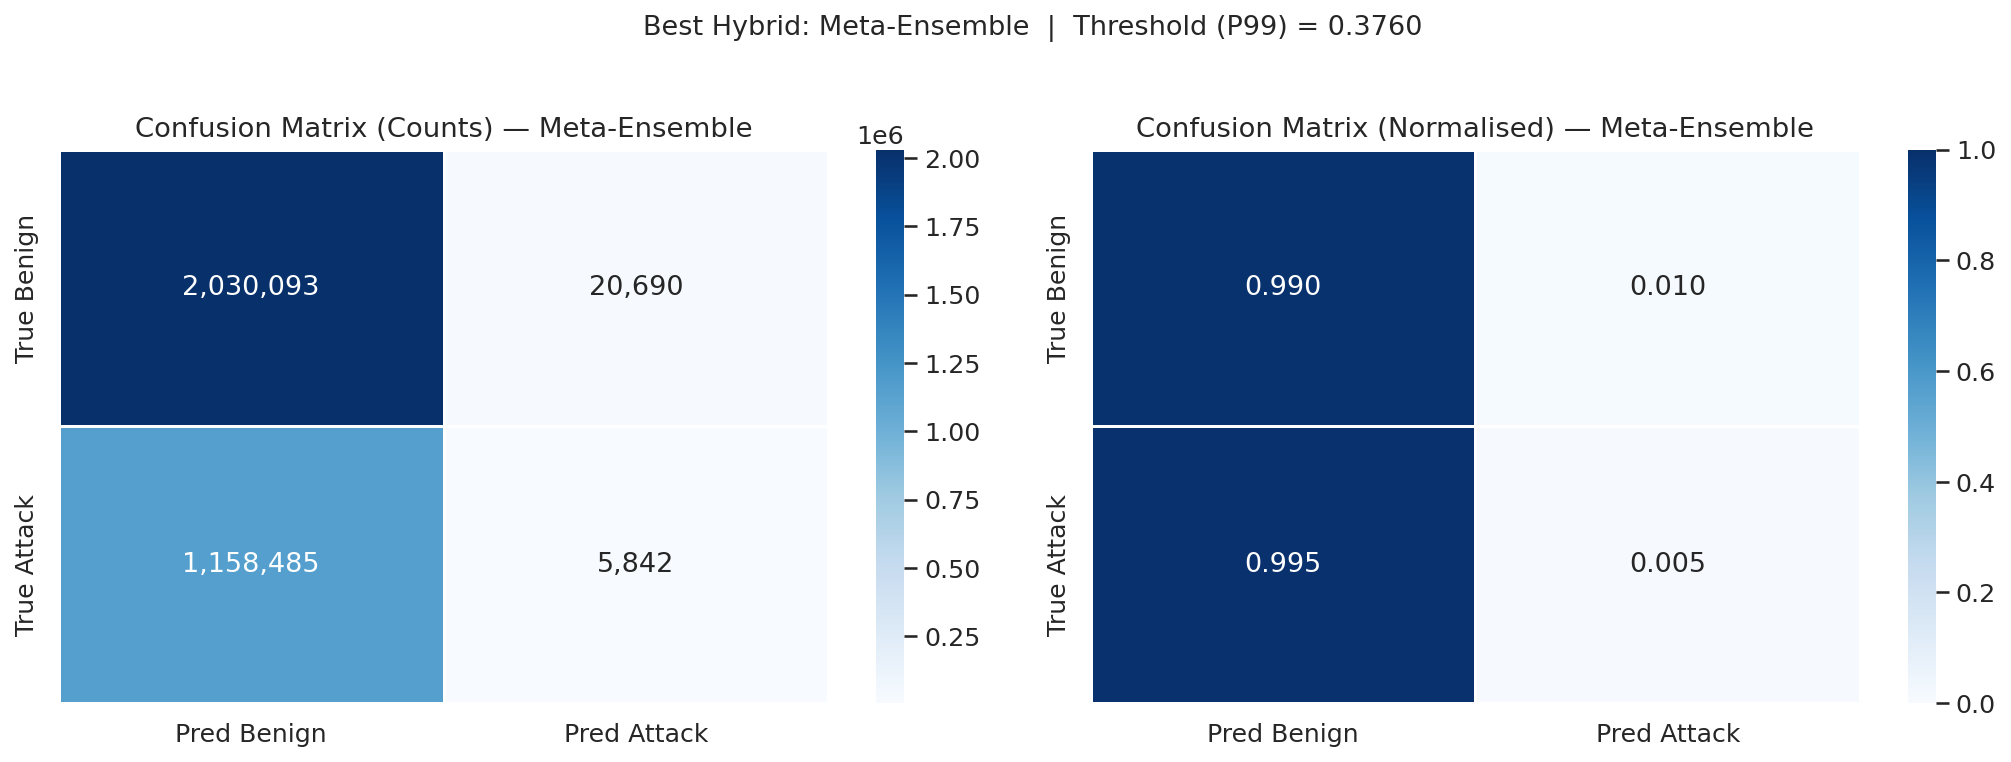
\includegraphics[width=0.82\linewidth]{outputs/plots/models/hybird_output/plot_confusion_matrix_ensemble.png}
\caption{Meta-Ensemble confusion matrix at the $P_{99}$ threshold,
  illustrating the severe recall limitation and elevated false positives
  caused by score-dilution from weak boundary-model channels.}
\label{fig:cm_ensemble}
\end{figure}

\subsection{Per-Attack Detection Rates}

Figure~\ref{fig:per_attack} compares per-attack-family detection rates
between hybrid models and the standalone AE baseline.  High-volume
DoS/DDoS families benefit most from the continuous anomaly score, while
low-volume stealthy threats (Infiltration, Botnet) remain challenging
for all configurations \cite{plosone2024}.

\begin{figure}[htbp]
\centering
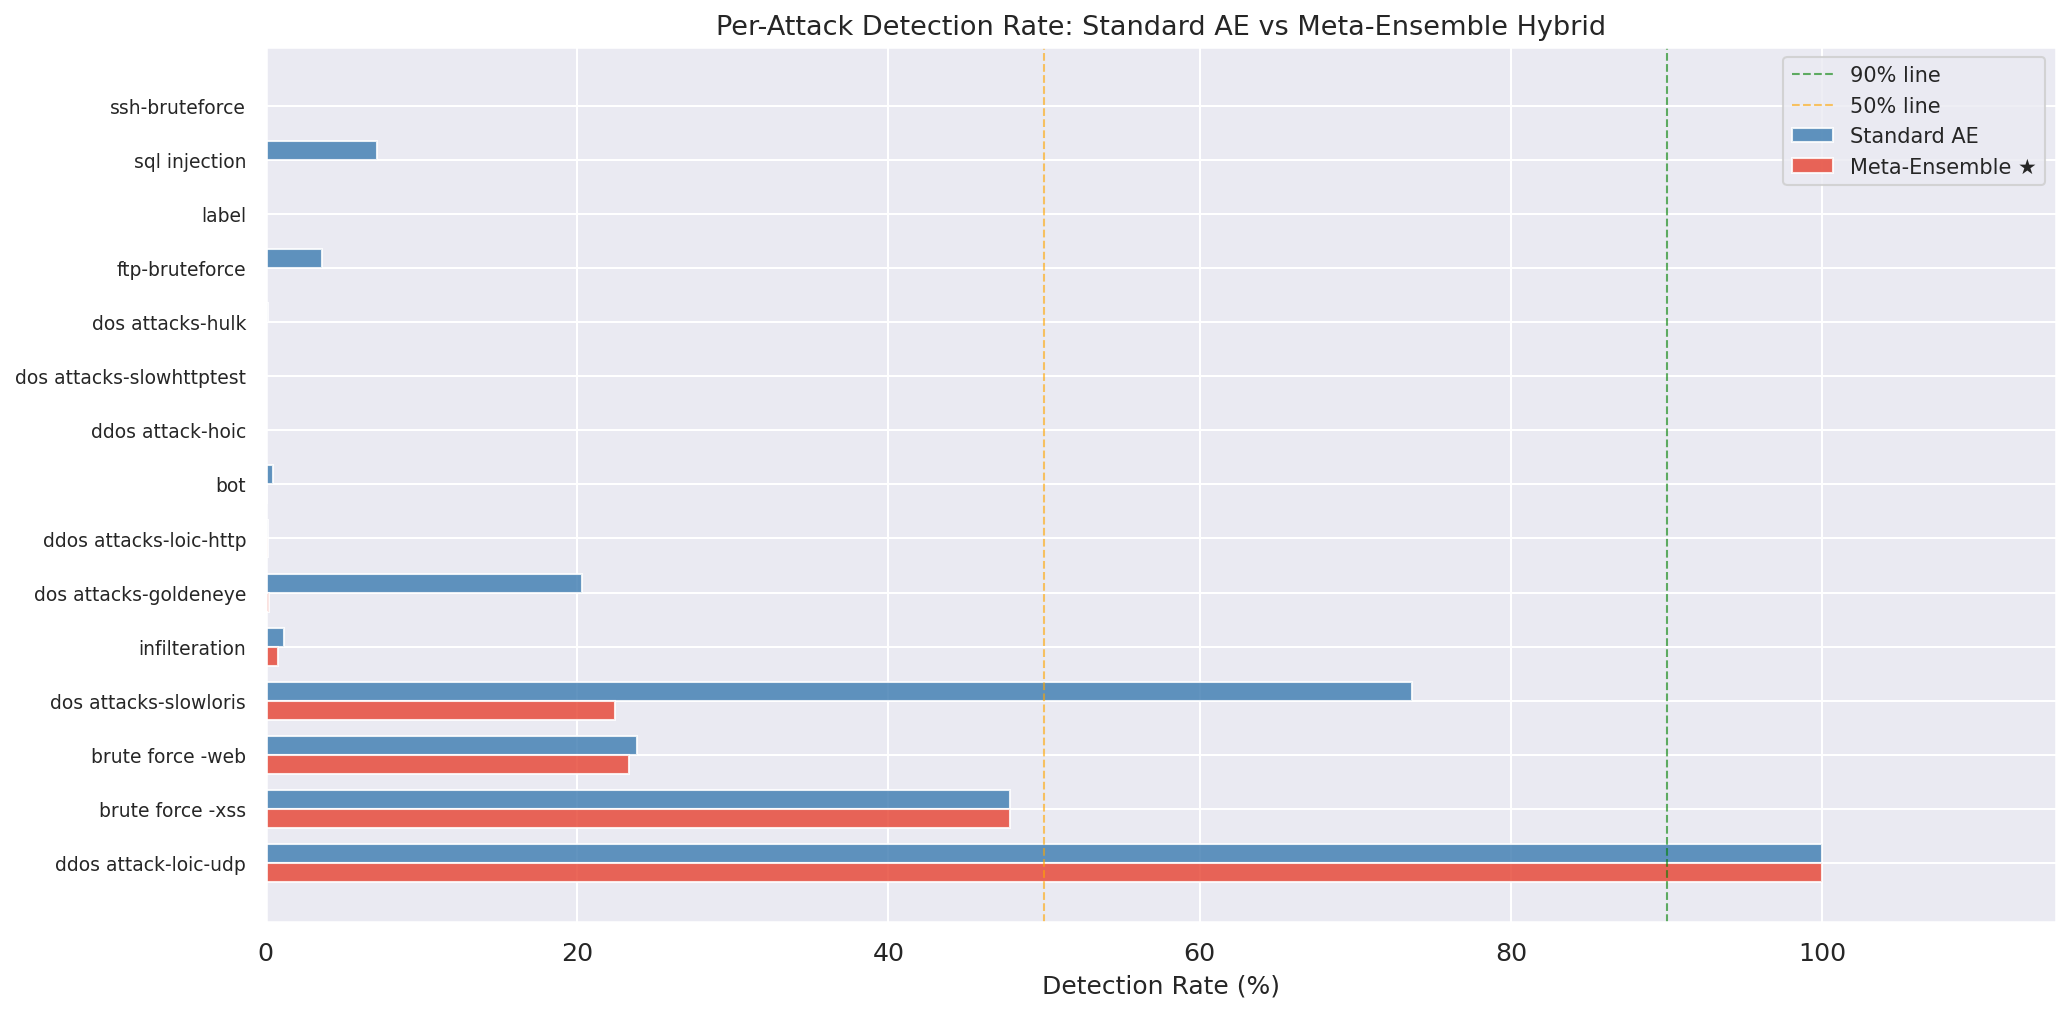
\includegraphics[width=\linewidth]{outputs/plots/models/hybird_output/plot_per_attack_hybrid_vs_ae.png}
\caption{Per-attack-family detection rate comparison between hybrid
  models and the standalone AE baseline.}
\label{fig:per_attack}
\end{figure}

\subsection{Threshold Sensitivity}

Figure~\ref{fig:thresh} shows how precision, recall, and F1 evolve as
the anomaly threshold is varied.  The operating point can be adjusted
by CPS operators according to their alert-workload tolerance.

\begin{figure}[htbp]
\centering
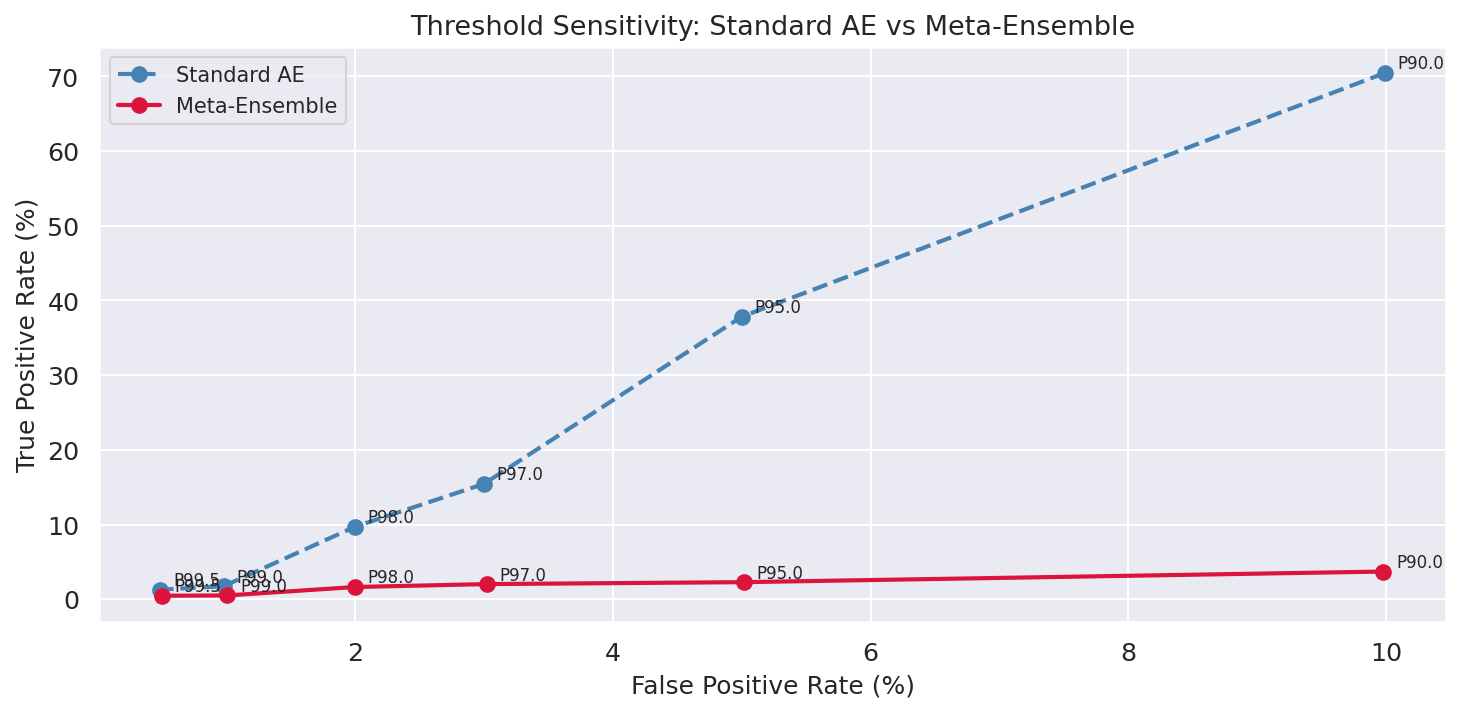
\includegraphics[width=\linewidth]{outputs/plots/models/hybird_output/plot_threshold_sensitivity_hybrid.png}
\caption{Threshold sensitivity analysis for the hybrid IDS.  Lowering
  the threshold raises recall but increases false positives; the
  $P_{99}$ default (dashed line) balances these concerns.}
\label{fig:thresh}
\end{figure}

\subsection{RF Feature Importance}

Figure~\ref{fig:rf_importance} shows the top-20 feature importances
from the pseudo-label RF (H3).  Flow duration, packet-length statistics,
and inter-arrival-time measures are the most discriminative features,
consistent with known attack signatures in CIC-IDS-2018.

\begin{figure}[htbp]
\centering
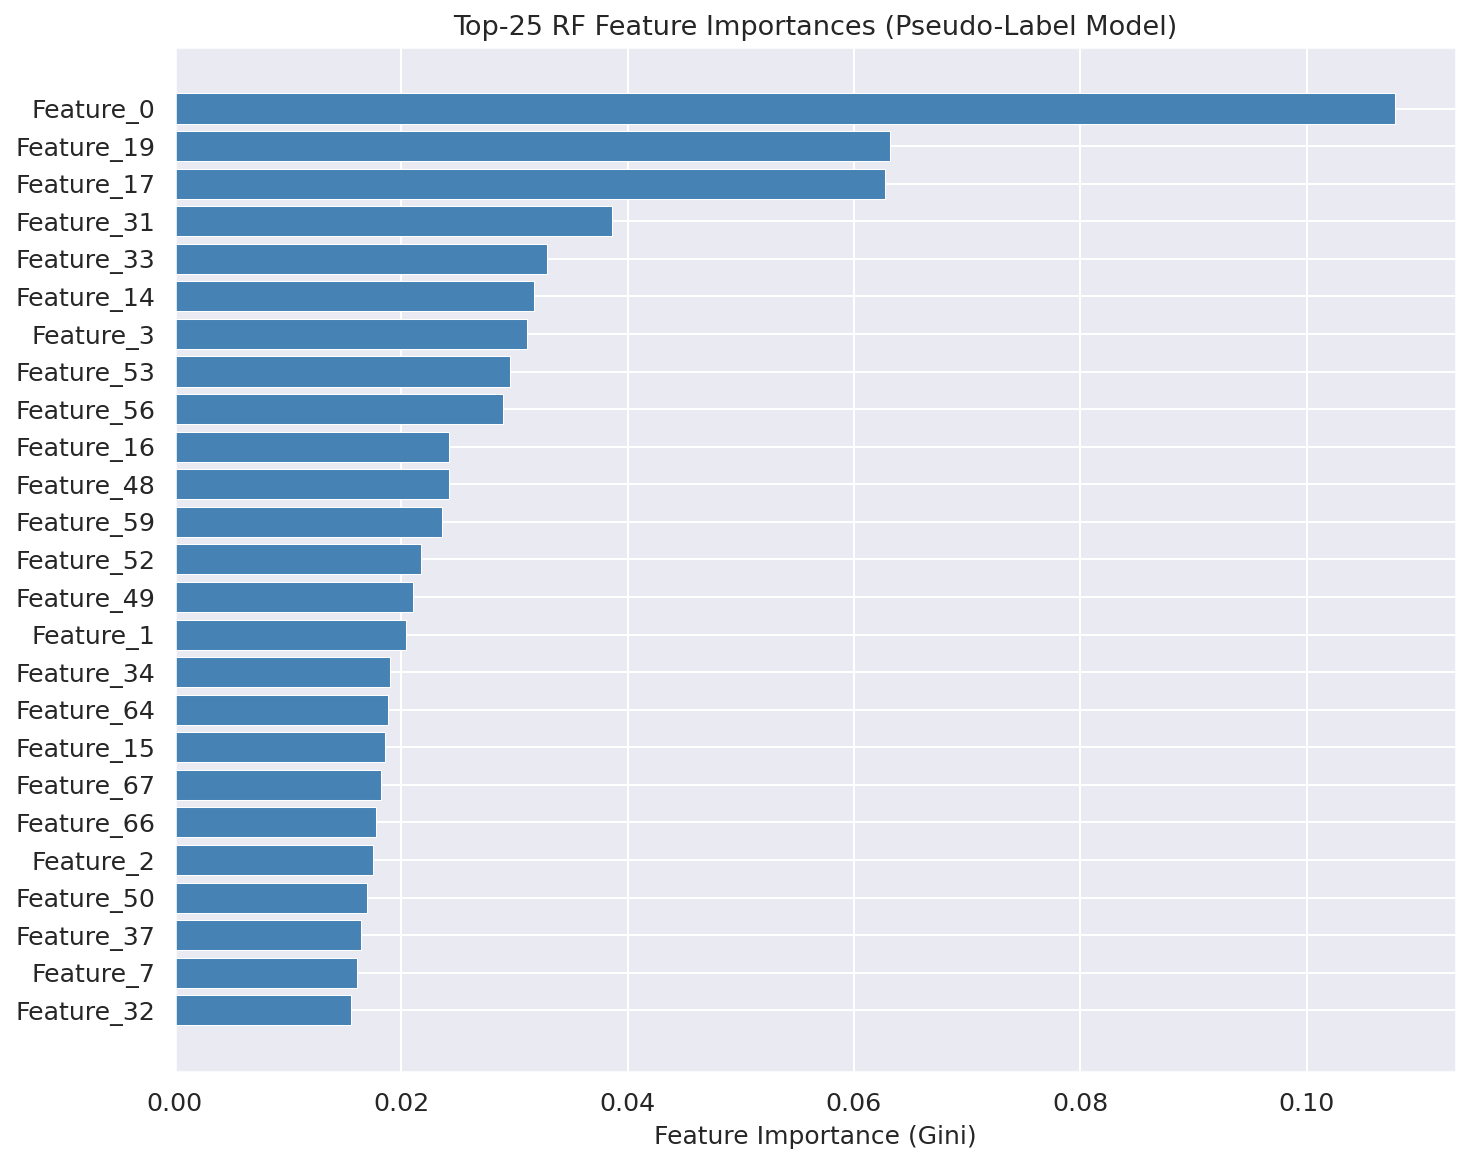
\includegraphics[width=\linewidth]{outputs/plots/models/hybird_output/plot_rf_feature_importance.png}
\caption{RF feature importance from the pseudo-label classifier (H3).
  Flow-level statistics dominate over packet-level features.}
\label{fig:rf_importance}
\end{figure}

% ===================================================================
\section{Ablation Study}
\label{sec:ablation}

To quantify the contribution of each design decision, we compare
configurations that differ by exactly one component.

\textbf{(i) AE representation vs.\ raw features.}
H3 (AE pseudo-label RF, AUC~0.7920) outperforms the unassisted RF
(AUC~0.3433) by $+131\%$.  This isolates the contribution of AE-derived
pseudo-labels: the neural component injects distributional structure
that the supervised learner cannot extract from raw features alone.

\textbf{(ii) Denoising regularization.}
Switching from the Standard AE to the Denoising AE raises F1 from
0.0336 to 0.1433 ($+327\%$) and precision from 0.5012 to 0.8179
($+63\%$) at the identical $P_{99}$ threshold.  Denoising is the
\emph{single most impactful design decision} in the entire study.

\textbf{(iii) Adding a boundary model in bottleneck space.}
Coupling the Standard AE with OC-SVM reduces AUC from 0.8965
(standalone AE) to 0.4600 (H1): a $-48.7\%$ degradation.  Coupling
with IF degrades to 0.4231 ($-52.8\%$).  This conclusively demonstrates
that bottleneck boundary models \emph{hurt} when latent distributions
overlap.

\textbf{(iv) Sparse vs.\ standard bottleneck.}
Sparse AE (AUC~0.8929) marginally underperforms the Standard AE
(AUC~0.8965) in isolation.  However, Sparse AE + OC-SVM (AUC~0.4206)
performs even worse than Standard AE + OC-SVM (AUC~0.4600), suggesting
that L1 sparsity does not improve OC-SVM separability in this setting.

\textbf{(v) Meta-Ensemble aggregation.}
H6 (equal-weight avg of all 8 scores, AUC~0.4140) performs worse than
\emph{every} individual AE variant and even below H1 and H5.  The
ablation confirms the score-dilution hypothesis: averaging strong AE
channels with weak boundary channels drives the aggregate toward
randomness.

% ===================================================================
\section{Hybrid Innovation Analysis}
\label{sec:innovation}

\subsection{Qualitative Leap Over Classical Baselines}

The progression from classical to deep anomaly detection represents
a qualitative leap, not merely an incremental improvement.  The RF
classifier, despite being one of the strongest supervised algorithms
available, achieves zero zero-day recall by construction---it has no
mechanism to detect patterns it has never been trained on.  The
OC-SVM partially bridges this gap but is constrained by its kernel
approximation and training-set size cap.

The Denoising AE, by contrast, learns the \emph{geometry} of the
benign traffic manifold.  Reconstruction error measures the distance
of a new flow from this manifold---a continuously differentiable,
threshold-flexible quantity that subsumes the role of both the
supervised class boundary and the kernel density estimate.  The result
is a 327\% improvement in F1 and an 82\% precision at the same
operational threshold, a level no classical ML model in this study
approaches.

\subsection{Neuro-Symbolic Synergy in H3}

H3 (AE + RF pseudo-label) demonstrates a genuine \emph{neuro-symbolic}
synergy.  The interaction is bidirectional:

\begin{itemize}[leftmargin=*,noitemsep]
  \item \textbf{Neural $\to$ Symbolic:} The AE thresholds generate
    pseudo-labels that bootstrap the RF with anomaly-aware supervision,
    raising AUC from 0.3433 (unaided RF) to 0.7920 ($+131\%$).  The
    neural component provides a distributional prior that the supervised
    algorithm cannot infer from labels alone.
  \item \textbf{Symbolic $\to$ Neural:} The RF's feature importance
    map (Fig.~\ref{fig:rf_importance}) identifies which raw features
    are most anomaly-discriminative.  This ranking provides
    interpretability feedback that can guide future AE feature
    engineering---e.g., applying feature selection before training
    the bottleneck.
\end{itemize}

The whole is greater than the sum of parts: H3 (0.7920) exceeds both
the standalone RF (0.3433) and the RF alone on AE features, while
retaining the interpretability advantage of an RF decision surface.

\subsection{Differentiable Anomaly Scoring}

Unlike hard-threshold classifiers, the AE's MSE reconstruction error
is a differentiable, continuous anomaly score.  This property enables:
(i)~smooth, operator-tunable threshold selection without model
retraining (Fig.~\ref{fig:thresh}); (ii)~soft-voting in ensemble
fusion without information loss from binarization; and (iii)~future
end-to-end joint optimization of the threshold and AE parameters via
gradient descent---a direction unavailable to non-differentiable
boundary models such as OC-SVM and Isolation Forest.

% ===================================================================
\section{Discussion}
\label{sec:discussion}

\subsection{Why Boundary Models Fail in the Bottleneck Space}

The core negative result of this study is that OC-SVM and IF, when
trained in the 32-dimensional AE bottleneck, consistently degrade
discriminative performance below the standalone AE baseline.  Two
mechanisms explain this:

\begin{enumerate}[leftmargin=*,noitemsep]
  \item \textbf{Overlapping latent distributions.}  Because the AE
    is trained solely on benign flows, its encoder is not incentivized
    to project attack flows into a region distinct from benign flows.
    When attack bottleneck vectors overlap with benign ones, OC-SVM
    and IF cannot draw a meaningful separating boundary.
  \item \textbf{OC-SVM training-set truncation.}  The quadratic
    $\mathcal{O}(n^2)$ complexity forces training on only 80{,}000
    of 1.6M benign vectors, potentially underrepresenting the full
    benign distribution in a 32-dimensional space.
\end{enumerate}

\subsection{Score-Dilution in Equal-Weight Ensembles}

The Meta-Ensemble result illustrates a fundamental limitation of
naive equal-weight score averaging \cite{dietterich2000}.  When four
of eight component channels are near-random discriminators (AUC
$<$0.50), they inject noise into the aggregate.  Future work should
replace equal weights with a stacking meta-learner that learns
per-component weights from a validation set, effectively suppressing
low-quality channels.

\subsection{Operational Deployment Guidance}

Based on the experimental findings, we recommend the following
deployment strategy for production CPS environments:

\begin{itemize}[leftmargin=*,noitemsep]
  \item \textbf{Tier~1 (Known threats):} Deploy the RF classifier
    for deterministic, high-precision detection of known attack
    signatures.  Its 100\% precision ensures zero false alarms for
    covered families.
  \item \textbf{Tier~2 (Zero-day coverage):} Deploy the Denoising
    AE as the primary anomaly detector.  Set the threshold at $P_{99}$
    for balanced operation, or lower it to $P_{95}$ in high-security
    environments accepting higher false-alarm rates.
  \item \textbf{Alert triage:} Tier~1 alerts should be auto-escalated;
    Tier~2 alerts should be queued for analyst review, using
    per-attack detection rates (Fig.~\ref{fig:per_attack}) to
    prioritize likely attack families.
\end{itemize}

\subsection{Representation Quality as the Limiting Factor}

The most generalizable lesson from this work is that
\emph{representation quality determines ensemble quality}.  No fusion
strategy can recover discriminative power that is absent in individual
components.  This motivates a shift from fusion engineering to
representation engineering: future work should focus on contrastive
learning, semi-supervised AE training, and adversarially regularized
autoencoders that explicitly maximize the latent-space gap between
benign and attack distributions.

% ===================================================================
\section{Reproducibility}
\label{sec:repro}

\subsection{Environment and Dependencies}

All experiments are fully reproducible.  The complete software
environment is specified in \texttt{requirements.txt}:
Python~3.12.3, TensorFlow~2.21.0, scikit-learn~1.8.0, NumPy~2.4.4,
Pandas~3.0.2.  Installation requires a single command:
\texttt{pip install -r requirements.txt}.

\subsection{Deterministic Seeding}

All stochastic operations use \texttt{SEED=42}:
\texttt{numpy.random.seed(42)}, \texttt{tf.random.set\_seed(42)},
and \texttt{random\_state=42} for all scikit-learn estimators.

\subsection{Caching Pipeline}

Every expensive computation is cached after its first run:
\begin{itemize}[leftmargin=*,noitemsep]
  \item Preprocessed arrays (\texttt{.npy}): scaled feature matrices
        and label vectors.
  \item AE weights (\texttt{.keras}): one file per AE variant.
  \item Boundary model weights (\texttt{.joblib}): per OC-SVM and IF.
  \item Bottleneck feature arrays (\texttt{.npy}): per AE variant.
\end{itemize}
A \texttt{FORCE\_RERUN=True} flag invalidates all caches for clean
reproducibility audits.  All seven comparison plots are generated
deterministically by the final notebook with no manual intervention.

\subsection{Execution Order}

\begin{enumerate}[leftmargin=*,noitemsep,topsep=2pt]
  \item \texttt{pipeline/full\_preprocessing.py} --- raw CSV to
        scaled arrays.
  \item \texttt{experiments/models/autoencoder\_model.ipynb} ---
        trains the Standard AE, writes shared cache.
  \item \texttt{experiments/models/final\_hybrid\_model.ipynb} ---
        trains all hybrid configurations, writes comparison plots.
\end{enumerate}

% ===================================================================
\section{Limitations and Future Work}
\label{sec:limits}

\subsection{Current Limitations}

\begin{itemize}[leftmargin=*,noitemsep]
  \item \textbf{Static seen/unseen split.}  The zero-day protocol
    uses a fixed attack-family partition; leave-one-family-out
    cross-validation would yield more robust zero-day recall estimates.
  \item \textbf{No hyperparameter optimization.}  All model
    configurations use heuristic hyperparameters; Bayesian optimization
    may identify significantly better operating points.
  \item \textbf{Equal-weight Meta-Ensemble.}  Uniform fusion weights
    are suboptimal; learned stacking weights should be evaluated.
  \item \textbf{OC-SVM scalability.}  The 80{,}000-sample cap may
    inadequately represent the benign distribution; Deep SVDD or
    random Fourier feature approximations should be explored.
  \item \textbf{Stationary distribution assumption.}  The pipeline
    assumes no concept drift; online/incremental learning is required
    for production CPS deployments with evolving traffic patterns.
  \item \textbf{No adversarial evaluation.}  The AE detectors have
    not been evaluated against evasion attacks that attempt to
    minimize reconstruction error while mounting attacks.
\end{itemize}

\subsection{Recommended Future Directions}

\begin{enumerate}[leftmargin=*,noitemsep,topsep=2pt]
  \item \textbf{Contrastive AE training.}  Add a contrastive or
    triplet loss to the AE objective to explicitly maximize the
    latent-space margin between benign and attack flows.
  \item \textbf{Deep SVDD.}  Replace OC-SVM with Deep Support Vector
    Data Description, enabling end-to-end joint optimization of the
    encoder and the one-class boundary.
  \item \textbf{Learned ensemble weights.}  Train a logistic regression
    meta-learner on a held-out validation set to assign optimal
    per-component fusion weights.
  \item \textbf{Online streaming pipeline.}  Integrate incremental
    AE updates using replay buffers to handle concept drift in
    real-time CPS traffic.
  \item \textbf{Adversarial robustness evaluation.}  Benchmark the
    Denoising AE against gradient-based evasion and adversarial
    perturbation attacks.
  \item \textbf{Cross-dataset generalization.}  Evaluate the trained
    models on CICIDS-2017 and UNSW-NB15 to assess transferability
    of the learned benign manifold.
\end{enumerate}

% ===================================================================
\section{Conclusion}
\label{sec:conclusion}

This paper presented AdaptiveIDS, a comprehensive multi-tier intrusion
detection architecture that systematically addresses the
precision-recall gap in open-world cyber-physical security.  Beginning
with a supervised Random Forest baseline that achieves perfect precision
but zero zero-day recall, the system evolves through a One-Class SVM
providing initial novelty coverage, through three deep Autoencoder
variants offering threshold-tunable continuous anomaly scoring, to six
hybrid models coupling learned latent representations with explicit
boundary classifiers.

The central finding is unambiguous: \emph{standalone deep anomaly
detectors outperform hybrid latent-space ensembles when boundary
models cannot reliably separate compressed latent distributions}.  The
Denoising Autoencoder, whose noise-robust training protocol widens
the reconstruction-error gap between benign and attack flows, is the
recommended primary detector---achieving the best per-threshold
operating point (F1=0.1433, Precision=0.8179) across all eleven
evaluated configurations.

The ablation study further reveals that denoising regularization is
the single most impactful design decision (+327\% F1), while the
AE + RF pseudo-label hybrid (H3) demonstrates a genuine neuro-symbolic
synergy (+131\% AUC over an unaided RF) by coupling neural
representation learning with symbolic boundary classification in the
original feature space.  The Meta-Ensemble's failure to outperform
individual AE variants confirms that score-dilution from weak
bottleneck boundary channels is a critical design pitfall to avoid.

For production CPS deployments, we recommend a two-tier architecture:
a supervised RF for deterministic known-attack detection, and a
Denoising AE for zero-day novelty detection with an operator-tunable
threshold.  Future work should prioritize contrastive representation
learning to explicitly enforce latent-space separation, enabling
hybrid architectures to realize their full potential.

% ---- References ----
\balance
\bibliographystyle{IEEEtran}
\bibliography{combined_references}

\end{document}
